\documentclass[conference]{IEEEtran}
\IEEEoverridecommandlockouts
% The preceding line is only needed to identify funding in the first footnote. If that is unneeded, please comment it out.
\usepackage{cite}
\usepackage{amsmath,amssymb,amsfonts}
\usepackage{algorithmic}
\usepackage{graphicx}
\usepackage{caption}
\usepackage{textcomp}
\usepackage{xcolor}
\usepackage[utf8]{inputenc}
\usepackage{tabularx}
\def\BibTeX{{\rm B\kern-.05em{\sc i\kern-.025em b}\kern-.08em
    T\kern-.1667em\lower.7ex\hbox{E}\kern-.125emX}}
\begin{document}

\title{Desenvolvimento De Drones e Sua Inserção Na Robótica Educacional}

%%\author{Gustavo da Silva Nascimento Costa$^{1}$, João Vitor Nascimento$^{2}$, Jeovana Miranda Souza$^{3}$, Rafael Gomes de \\ Oliveira$^{4}$, Sávio Pessôa Afonso$^{5}$, Rian Cesar Oliveira Souza$^{6}$, Leandro Gonçalves dos Santos$^{7}$, \\and Fábio Santos Lima$^{8}$}

\maketitle

\begin{abstract}
O projeto Educa Drones do Instituto Federal Baiano - Campus Guanambi utiliza a tecnologia STEAM em um contexto interdisciplinar de robótica educacional, focando em drones de asa rotativa como o IF450 e as versões Colibri, todos de open-hardware. Estudantes e professores podem explorar conceitos complexos construindo e operando esses drones, que são modelados em Tinkercad, impressos em 3D com polímero PETG, e possuem design modular e robusto, com componentes eletrônicos avançados e telemetria via rádio ESP32. A iniciativa melhora o aprendizado, incentiva o empreendedorismo e inovação, e introduz um novo modelo de negócio no cenário acadêmico e empresarial.
\end{abstract}

\begin{IEEEkeywords}
Aeronave remotamente pilotada, robótica educacional, F450, multirotor, quadricoptero, modularidade.
\end{IEEEkeywords}

\section{Introdução}

Atualmente, o Brasil apresenta diversos problemas relacionados à defasagem do sistema público educacional, como mostram os resultados do Programa Internacional de Avaliação dos Estudantes (PISA, 2023), onde mais de 50\% dos adolescentes de 15 anos não possuem nível básico de conhecimento em matemática, ciências e linguagens \cite{b6}. Situação que vem se agravando desde 2009.

Diante de tal fato, faz-se necessário a procura de meios que incentivem o aprendizado dos alunos. Dessa forma, a utilização de recursos tecnológicos com finalidades pedagógicas em instituições de ensino, vem despertando interesse crescente na busca por ferramentas que auxiliem no processo de ensino e aprendizagem \cite{b12}.

Na chamada robótica educacional, um desses recursos tecnológicos  utilizados para incentivar o interesse do aluno é a aeronave remotamente pilotada, conhecida popularmente por drone. Através dele é possível explorar conceitos da física e matemática, tais como dinâmica do voo, força, empuxo e leis de Newton, distância, altura, ângulos, trigonometria, dentre outros \cite{b11}. Conteúdos estes, que se mostram difíceis de assimilar dentro do paradigma de ensino tradicional.

Além disso, através da construção desses dispositivos é possível entender e aplicar conceitos básicos e avançados de eletrônica, química, engenharia e programação \cite{b12}. Noções fundamentais na capacitação de profissionais que serão inseridos em um mercado globalizado. Desta perspectiva, nasceu no Instituto Federal de Educação, Ciência e Tecnologia Baiano - Campus Guanambi, localizado no sertão produtivo, o projeto Educa Drones, uma iniciativa pioneira no cenário estadual. Promovendo através de oficinas, palestras, competições estudantis, empreendedorismo e da inovação tecnológica, um ambiente estimulante e colaborativo para que professores e estudantes se capacitem, troquem experiências e comparti\-lhem ideias que resultem no desenvolvimento de drones e sua inserção no ensino e outros setores que requeiram sua utilização.

Seguindo essa linha de pensamento, através do Educa Drones, idealizou-se o subprojeto de iniciação científica “Desenvolvimento de drones e sua inserção na robótica Educacional”. Pensado inicialmente para o desenvolvimento do drone IF450, projetado para ser modular, resistente  e com alto desempenho, evoluiu para o desenvolvimento dos drones Colibri (standard, lite, mini, micro e hexa), com finalidades semelhantes, porém estruturados para o ensino. Incentivando através de palestras e oficinas a criação de projetos similares em outras instituições.

Tendo esses drones concebidos como produtos tecnológicos de interesse de um público nichado, essa iniciativa tem buscado estimular o empreendedorismo na instituição, a partir da criação de uma startup que possa explorar comercialmente esses drones desenvolvidos. As melhorias implementadas e características peculiares dos drones IF450 e da linha Colibri, apresentam-se como diferenciais competitivos interessantes que aliado a estratégias bem formuladas, podem se transformar num modelo de negócio atraente aos estudantes e demais integrantes do projeto. 

Para elaborar melhor esses aspectos, este artigo está organizado da seguinte forma. A Seção 2 apresenta o Referencial Teórico; A Seção 3 detalha os Materiais e Métodos; A Seção 4 apresenta os Resultados obtidos; E, por fim, a Seção 6 discute as conclusões do projeto.

\section{Referencial Teórico}

\subsection{Robótica Educacional}

A robótica educativa pode ser definida como uma área do conhecimento multidisciplinar que utiliza os conceitos das engenharias e demais ciências no processo de concepção, construção, automação e controle de dispositivos robóticos com propósitos educacionais \cite{b1}.

A utilização desses recursos tecnológicos com finalidades pedagógicas em instituições de ensino, vem despertando interesse crescente na busca por ferramentas que auxiliem no processo de ensino e aprendizagem \cite{b12}. No que se refere aos drones na educação, deve-se partir do princípio que a educação é um campo em constante evolução e inovação. Entretanto, observa-se uma insuficiência e um processo muito tímido sobre estudos científicos que contemplem a aplicação dos drones no ambiente pedagógico \cite{b9}.

Corroborando com esse entendimento, Yepes \cite{b11} afirma que há muito material sobre robótica educativa, entretanto, são raros os que focam o uso de drones na educação.  Na robótica educacional o drone pode ser utilizado como uma ferramenta de apoio ao ensino, explorando conceitos da física e matemática, tais como dinâmica do voo, força, empuxo e Leis de Newton, distância, altura, ângulos, trigonometria, dentre outros \cite{b11}.

\subsection{Legislação Brasileira Sobre Drones}

De acordo com Regulamento Brasileiro da Aviação Civil (RBAC-E n.94) os drones que possuem peso máximo de decolagem entre 250 g e 25 kg, que operam até 400 pés (cerca de 120 metros) acima do nível do solo e em linha de visada visual (VLOS) são classificados como classe 3 \cite{b2}.

Ainda de acordo com a ANAC, os drones dessa classe não precisam ser de um projeto autorizado ou tipo certificado por esse órgão, ou seja, não é necessário obter certificado de aeronavegabilidade, sendo exigido para sua operação o registro do operador e da aeronave no Sistema de Aeronaves não Tripuladas (SISANT), atender as regras constantes no RBAC-E n.94, assim como a conformidade com Agência Nacional de Telecomunicações (ANATEL) e autorização de voo pelo Departamento de Controle do Espaço Aéreo (DECEA).
\cite{b2}.

\subsection{Competições Estudantis}

Por conseguinte, surgem as competições de drones, tanto no âmbito acadêmico quanto no corporativo, que são um ambiente propício para o emprego da robótica educacional. Dentre elas pode-se citar a Fórmula Drone SAE Brasil,  a Drones IFSC, a Competição Brasileira de Robótica e a mais recente delas, a Competição Baiana de Drones.

A Fórmula Drone SAE Brasil é uma competição de caráter educacional tendo por objeto de interesse técnico o desenvolvimento de uma aeronave de asas rotativas rádio controlada, tipo drone, dotada de sistemas orientados para o cumprimento de determinadas tarefas que constituem o desafio técnico da competição, com foco tecnológico em sistemas inteligentes de bordo \cite{b7}. Foram realizadas três edições (2017, 2018 e 2019) da Fórmula Drones SAE Brasil que ocorreram no Campus da UNIFEI, cidade de Itajubá - MG, e teve sua sequência interrompida pela pandemia do COVID-19. Recentemente, a SAE Brasil divulgou em seu site, a retomada da competição para 2025 que agora tem um novo nome, EletroQuad, e será realizada na Universidade do Vale do Paraíba, em São José dos Campos.

A Competição de Drones do IFSC Campus Florianópolis, é realizada anualmente durante a Semana Nacional de Ciência e Tecnologia (SNCT), ocorrendo desde 2021, tem caráter educacional, com aplicação direta do conceito de STEAM (Science, Technology, Engineering, Arts, Mathematics) em uma atividade de desenvolvimento técnico e tecnológico voltada principalmente para alunos do ensino médio e graduação. O objetivo da competição é estimular os participantes a projetar, montar e pilotar um drone multirotor alimentado à bateria, além de realizar uma série de tarefas atualizadas pelo regulamento todos os anos, que desafiam as habilidades de resolução de tarefas dos participantes e as próprias capacidades técnicas dos veículos. O desempenho dos participantes é julgado através de regras pré-estabelecidas no regulamento da competição \cite{b4}.

A MNR é a maior Mostra Científica de trabalhos de robótica do país. É voltada para alunos do ensino fundamental, médio, técnico e alunos de Graduação, pós-graduação ou pesquisadores da área com o objetivo de estimular, expor e divulgar estudos e a pesquisa na área da Robótica. Os projetos mais bem avaliados concorrem a bolsas de Iniciação Científica Júnior CNPQ/MNR, sendo este projeto, um dos 60 premiados em todo Brasil na edição de 2023 \cite{b5}.

A Competição Brasileira de Robótica (CBR) é composta por 16 categorias que reproduzem problemas do cotidiano, onde robôs autônomos (sem qualquer intervenção humana) devem realizar tarefas corretamente. Entre as categorias, destaca-se a RoboCup Flying Robots League, que é uma modalidade de drones autônomos e inteligentes voltados para inspeção e operação em faixas de dutos e instalações \cite{b3}. Modalidade esta que terá a participação da equipe Drones Guanambi, a qual fará a utilização do drone Colibri Mini, que encontra-se em desenvolvimento e será fruto desse projeto, e que terá sua primeira aparição pública neste evento.

\subsection{Manufatura Aditiva}

A manufatura aditiva é uma ferramenta tecnológica que muito pode contribuir para a aplicação da robótica educacional. Seu conceito foi introduzido em meados da década de 1980 com a disseminação de metodologias de processos de prototipagem rápida, e a impressão tridimensional (3D) era um dos processos possíveis \cite{b10}.

A Impressão 3D é basicamente o ato de transformar uma matéria prima de uma condição física em outra, para produção de um objeto, tomando como base um modelo tridimensional que será materializado pela deposição de camadas \cite{b8}.

\section{Materiais e Métodos}

As aeronaves remotamente pilotadas podem ser do tipo asa fixa ou asa rotativa. Neste estudo nos limitamos ao tipo asa rotativa que também são chamados de multirrotores. Para fins de padronização, nos referimos a essas aeronaves usando o termo drone, como popularmente são conhecidas.

Tendo isso em vista, nesta seção serão explorados a construção da estrutura e a definição dos componentes eletrônicos dos drones desenvolvidos neste subprojeto abarcado pelo projeto Educa Drones. Esses modelos de iniciativa open-hardware foram denominados IF450, Colibri Standard, Colibri Lite, Colibri Mini, Colibri Micro e Colibri Hexa.


\subsection{Processo de Construção}

O drone genérico modelo F450 foi o ponto de partida para o desenvolvimento das novas aeronaves. Ele possui quatro braços de plástico injetado, fixados por parafos em duas placas de fibra de vidro para compor o \textit{frame}. Neste modelo, todos os componentes ficam expostos, a fiação é aparente e a aerodinâmica é prejudicada. Entretanto, apesar dos defeitos, trata-se de uma opção de baixo custo, consideravelmente leve e resistente, sendo amplamente utilizada em competições. 

\begin{figure}[!htb]
    \centering
    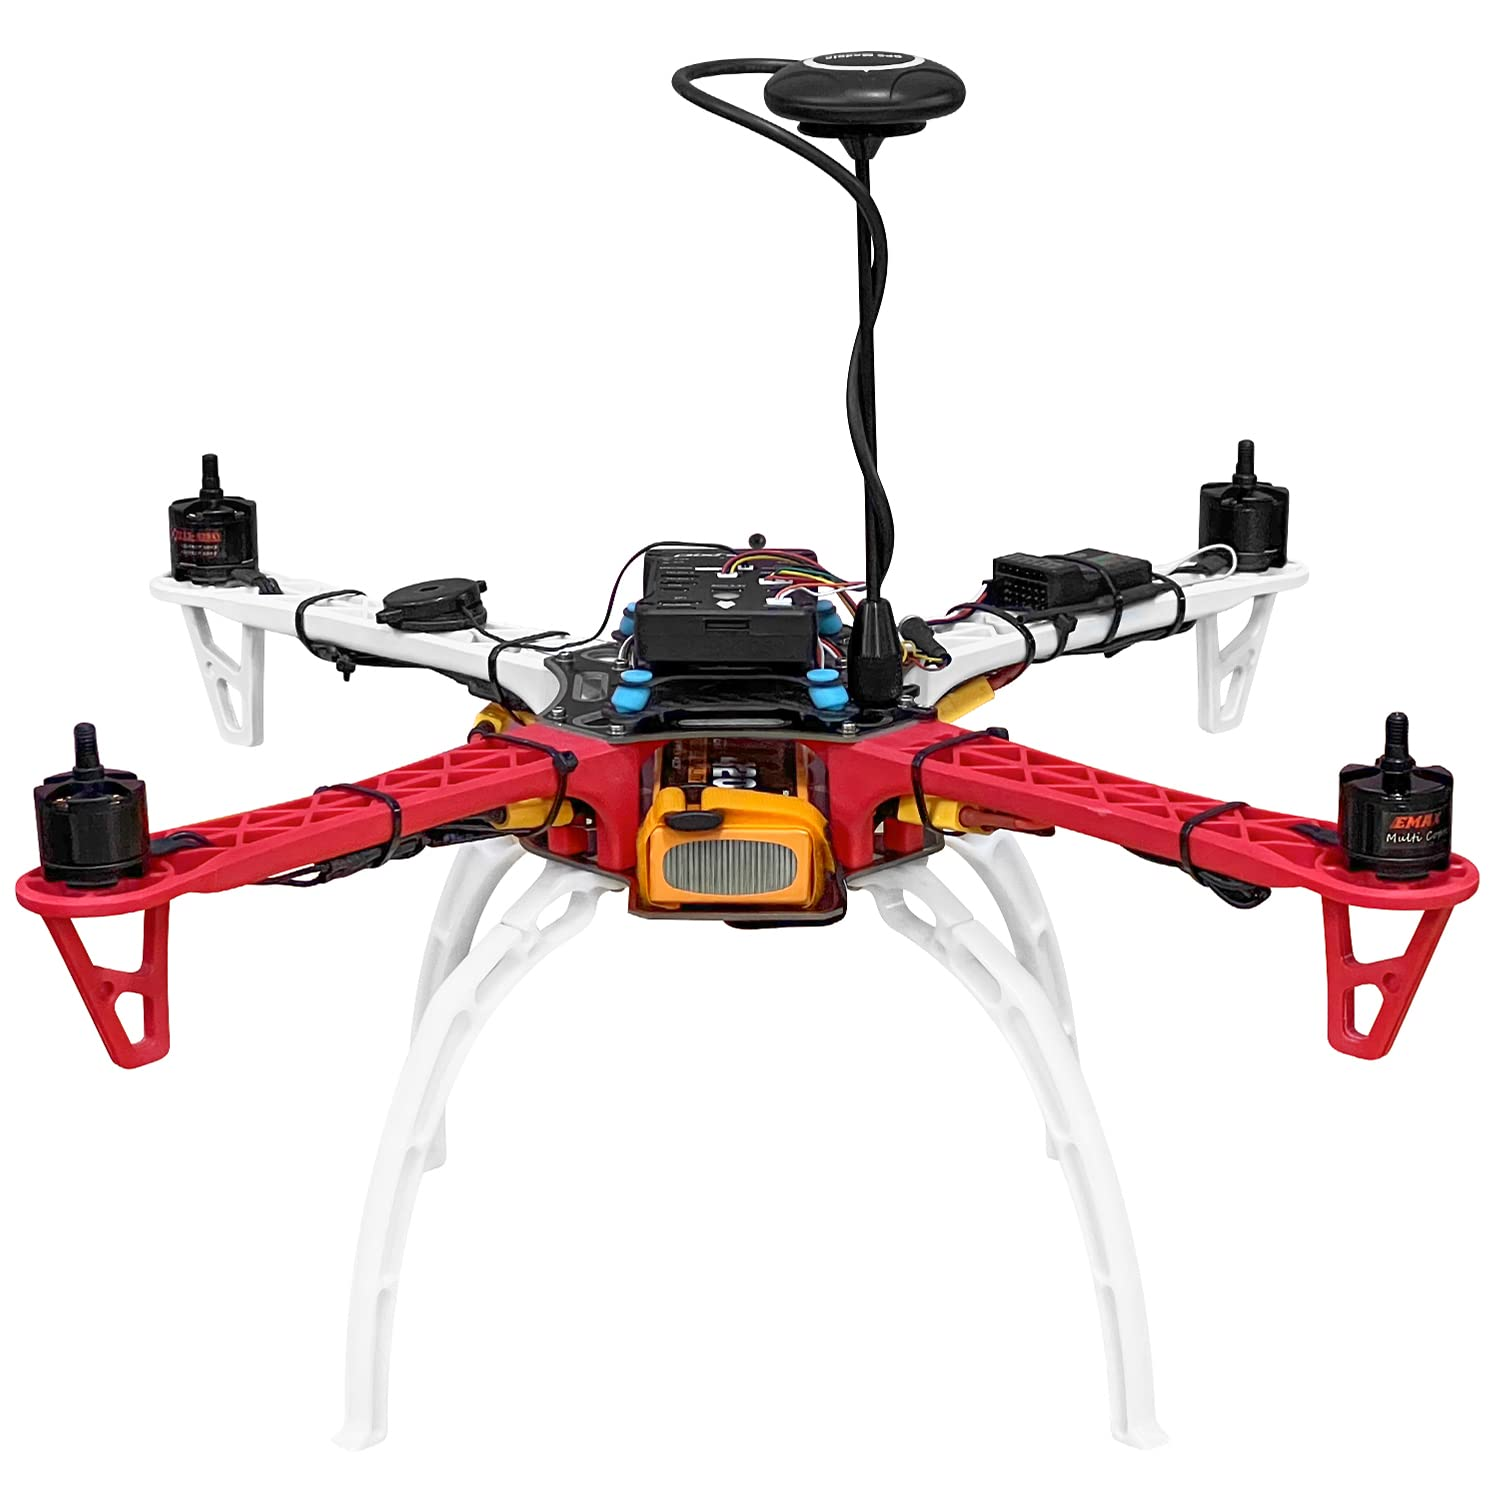
\includegraphics[scale=0.07]{img/f450.jpg} 
    \caption{Imagem do modelo F450 genérico. Fonte: Drones Company.}
    \label{fig:F450}
\end{figure}

Após Compreender suas limitações, iniciou-se a modelagem de drones que corrigissem suas falhas, mantendo sua proposta de ser leve, resistente e de baixo custo. Além disso, foi incluído o critério de modularidade para facilitar a troca de equipamentos, bem como um compartimento seguro e apropriado para o encaixe das baterias. A modelagem tridimensional foi desenvolvida na plataforma Tinkercad, uma ferramenta online gratuita, que pode ser acessado pelo navegador de internet e não exige uma máquina robusta para sua operação.

Após a confecção das peças, O arquivo do projeto foi exportado em formato “.STL" para ser fatiado em camadas, no programa FlashPrint. Ele é responsável por criar o arquivo com extensão “.GX” que é reconhecido pela impressora para realizar a extrusão camada por camada até finalizar a manufatura do objeto projetado.

As novas peças foram impressas em polímero PETG utilizando as impressoras Guider IIs, do fabricante Flash Forge, e a impressora A2v2 Core, da fabricante GTMax3D. O filamento PETG foi escolhido por agregar aos objetos manufaturados, características como durabilidade, tenacidade, flexibilidade, leveza e resistência à impactos.

\subsection{Modelo IF450}

\begin{figure}[!htb]
    \centering
    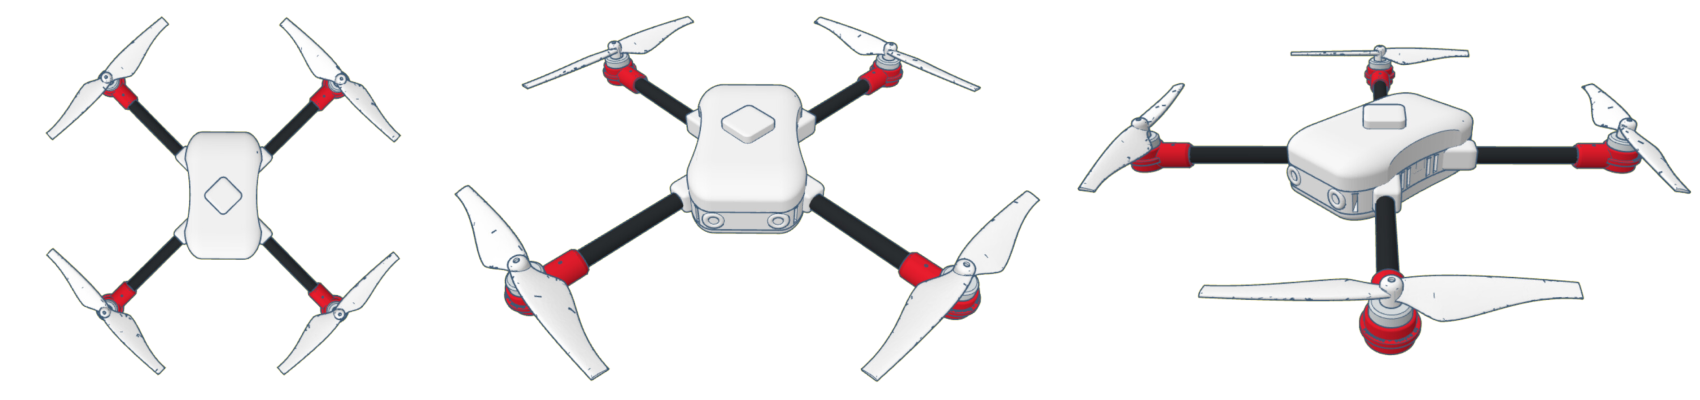
\includegraphics[scale=0.14]{img/IF450.png} 
    \caption{Modelo tridimensional do drone IF450 no TinkerCad. Fonte: o autor}
    \label{fig:IF450}
\end{figure}

Como mostrado na figura \ref{fig:IF450}, o modelo foi confeccionado com sua estrutura fechada com bordas arredondadas, aumentando a proteção de dispositivos e melhorando sua aerodinâmica. Possui braços feitos de tubos de fibra de carbono de 16 mm de diâmetro e parede interna de 1 mm, entradas e saídas de ar para permitir o arrefecimento do sistema eletro-eletrônico e encaixe apropriado de todos os equipamentos obrigatórios e acessórios periféricos. 

O novo drone foi denominado IF450, por representar o nome abreviado da instituição em que foi desenvolvido (IF de Instituto Federal) e 450 devido ao seu tamanho (distância entre os eixos do motor). Verifica-se que o centro do \textit{frame} é composto de uma peça inteiriça onde os braços de tubo de carbono se encaixam e onde a bateria é acoplada. Duas tampas, uma superior e outra inferior são fixadas por conectores de engate rápido e opcionalmente quatro parafusos de 2,5 mm de diâmetro. 

Com a remoção dessas tampas tem-se acesso rápido e facilitado da eletrônica interna em caso de necessidade de manutenção. Além de garantir aerodinâmica e proteção, mantém um visual limpo e elegante.

\subsection{Modelo Colibri Standard}

O drone recebe o nome de um beija-flor: Colibri, em homenagem à cidade de Guanambi (beija-flor em Tupi), tendo seu sufixo standard (“padrão” em inglês) por ser o modelo de referência para as demais versões. Seu formato é similar ao F450 genérico (figura \ref{fig:F450}).

\begin{figure}[!htb]
    \centering
    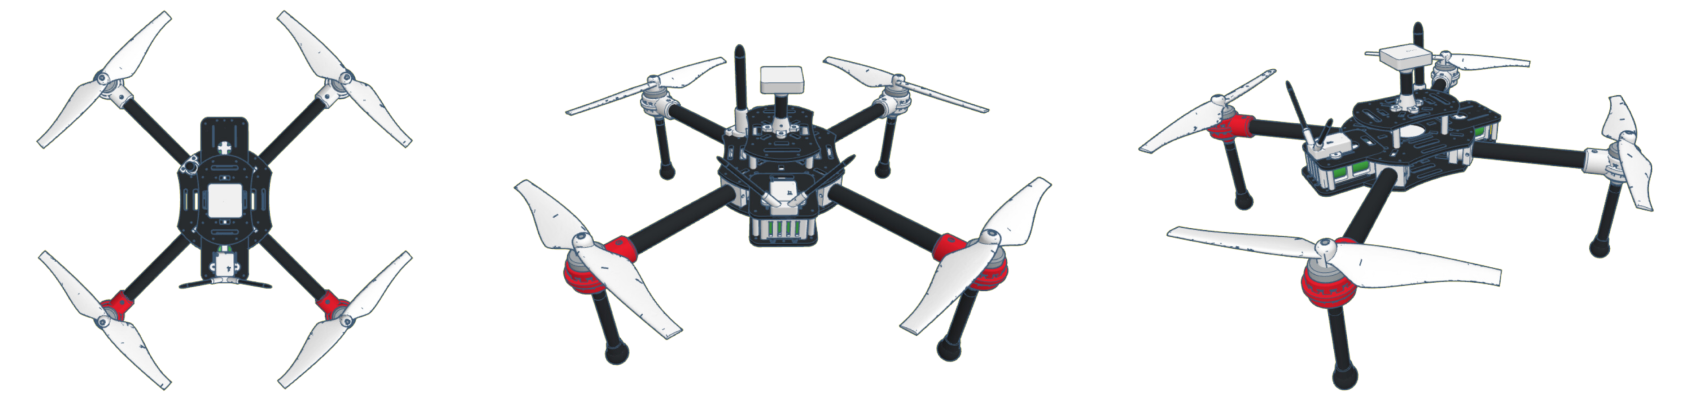
\includegraphics[scale=0.14]{img/Colibri-standard.png} 
    \caption{Modelo tridimensional do drone Colibri Standard no TinkerCad. Fonte: Autor}
    \label{fig:ColibriStandard}
\end{figure}

Ele mantém a distância de 450 mm entre os eixos e um centro de formato similar, utilizando braços tubulares de fibra de carbono, os mesmos do IF450, o que proporciona proteção para fios e dispositivos que podem ser inseridos em seu interior. O trem de pouso também é produzido com tubos de fibra de carbono, com 12 mm de diâmetro e 1 mm de espessura. 

Além disso, possui diversas furações previamente definidas que permitem a integração de variados acessórios como sensores e mecanismos robóticos.

\subsection{Modelo Colibri Lite}

O Colibri Lite possui as mesmas dimensões de sua versão \textit{Standard}, porém removendo diversas funcionalidades para priorizar a leveza. Ele foi planejado para competições nas quais o peso influencia significativamente na pontuação, mas que não permitem drones de dimensões menores.

\begin{figure}[!htb]
    \centering
    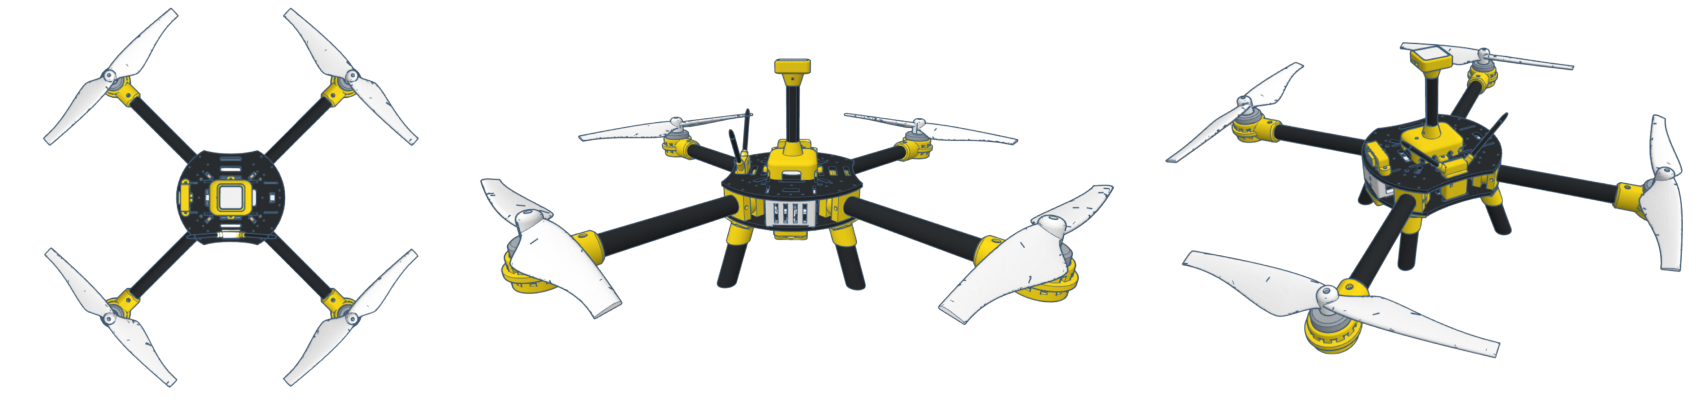
\includegraphics[scale=0.14]{img/Colibri-lite.png} 
    \caption{Modelo tridimensional do drone Colibri Lite no TinkerCad. Fonte: Autor}
    \label{fig:my_label}
\end{figure}

\subsection{Modelo Colibri Mini}
O Colibri Mini é um modelo que possui 330 mm entre os eixos dos motores. Ele apresenta braços de fibra de carbono tubulares de 12 mm de diâmetro e 1 mm de espessura, tratando-se de forma geral, um modelo em escala reduzida do Colibri Standard. 

Seu desenvolvimento foi iniciado pensando na utilização em competições onde apenas é permitido drones de tamanhos inferiores a 450 mm. Mesmo tendo por padrão 330 mm, essa dimensão pode ser modificada de acordo com a necessidade.

\begin{figure}[!htb]
    \centering
    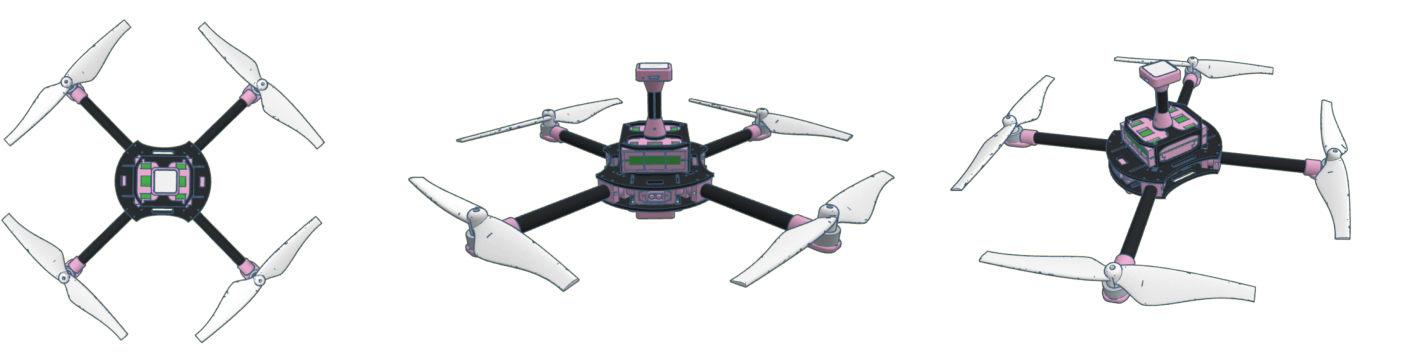
\includegraphics[scale=0.14]{img/Colibri-mini.png} 
    \caption{Modelo tridimensional do drone Colibri Mini no TinkerCad. Fonte: Autor}
    \label{fig:ColibriMini}
\end{figure}

\subsection{Modelo Colibri Micro}

O Colibri Micro é o modelo mais compacto e leve da série Colibri, com uma distância de 188 mm entre os eixos dos motores. Ele é o único a apresentar estrutura inteiramente feita por manufatura aditiva.

Desenvolvido para missões aéreas em locais fechados ou com demasiado obstáculos, onde sua proteção de hélice robusta e integrada nativamente permite menor vulnerabilidade a avarias e maior segurança à animais e pessoas

\begin{figure}[!htb]
    \centering
    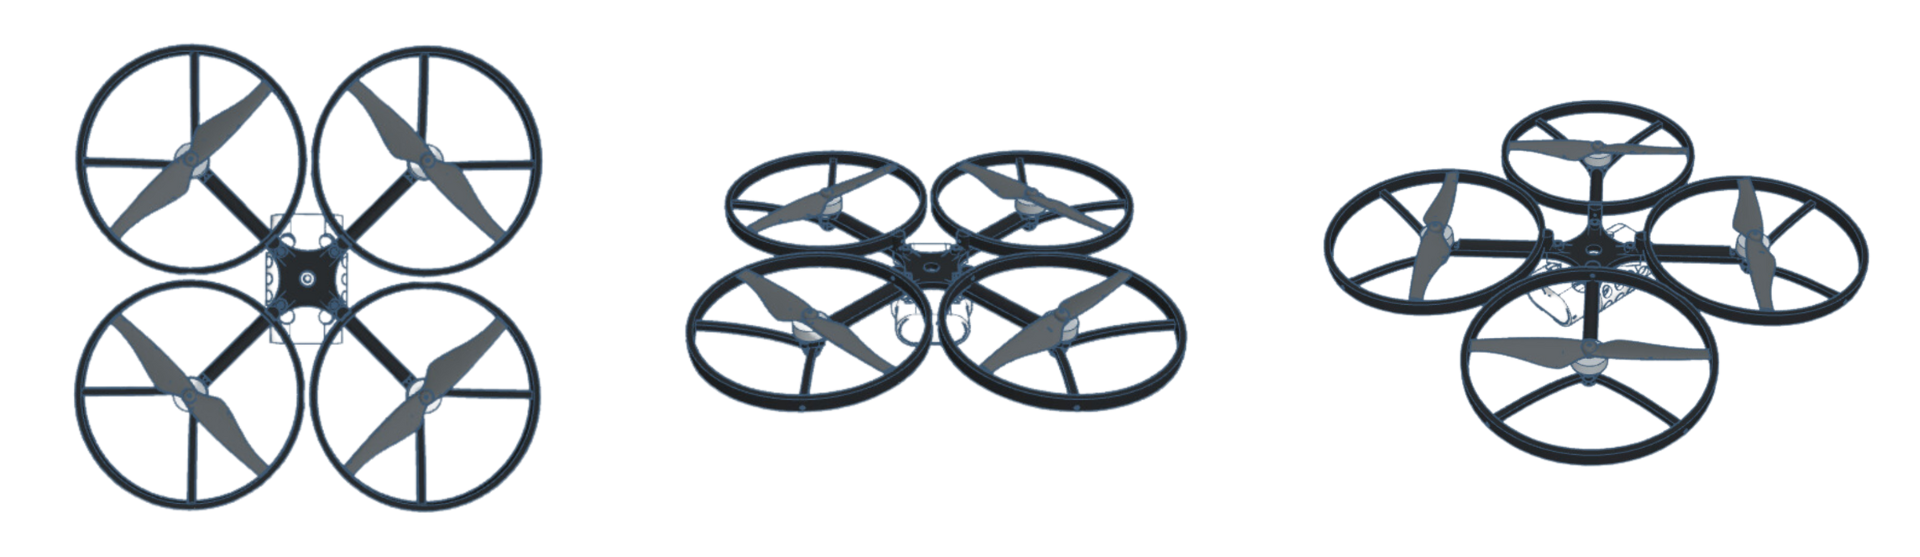
\includegraphics[scale=0.12]{img/Colibri-micro.png} 
    \caption{Modelo tridimensional do drone Colibri Micro no TinkerCad. Fonte: Autor}
    \label{fig:my_label}
\end{figure}

\subsection{Modelo Colibri Hexa}
O Colibri-Hexa é o maior de sua linha, com 6 rotores e 550mm de distância entre os opostos e 60° entre cada braço subsequente. Assim como nas outras versões, esse modelo possui braços tubulares de fibra de carbono com 16 mm de diâmetro.

\begin{figure}[!htb]
    \centering
    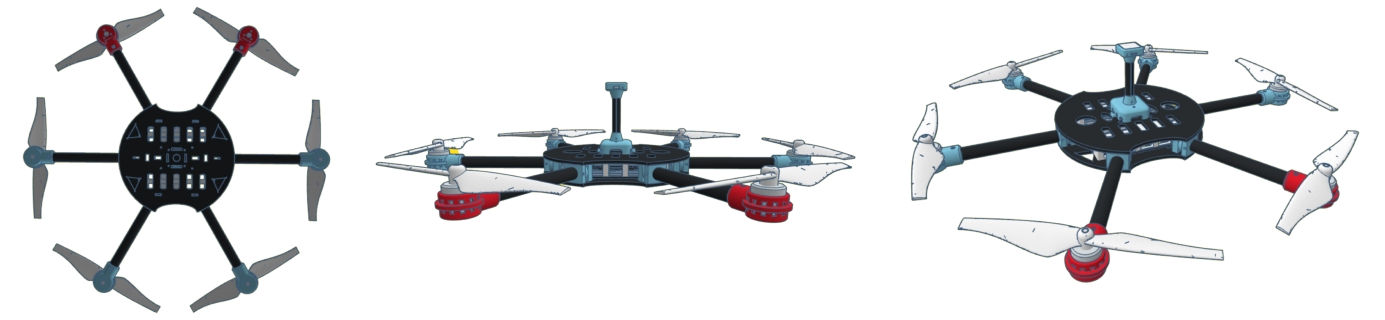
\includegraphics[scale=0.14]{img/Colibri-hexa.png} 
    \caption{Modelo tridimensional do drone Colibri Hexa no TinkerCad. Fonte: Autor}
    \label{fig:my_label}
\end{figure}

A existência de seis motores proporciona ao drone maior estabilidade e redundância, permitindo que a aeronave permaneça em voo mesmo com a falha de um deles. Ademais, ela é capaz de operar com peso adicional, o que possibilita a integração de equipamentos mais robustos.

\subsection{Componentes Eletrônicos}

Esse tópico aborda brevemente e de forma mais técnica o sistema de propulsão, controladoras de voo, sensores integrados e outros componentes essenciais que contribuem para a funcionalidade e desempenho dessas aeronaves não tripuladas.

Todas as versões de drones desenvolvidas compartilham componentes eletrônicos semelhantes, como o Electronic Speed Control (ESC), que utiliza o firmware BLHeli ou SimonK, e é conectado a uma controladora de voo de 32 bits configurada com o firmware Ardupilot.

Sobre aos rotores, são utilizados motores brushless de 800 KV, 1400 KV e 2824 KV, com uma relação inversamente proporcional ao tamanho da estrutura e da hélice.

Todas as baterias são desenvolvidas de maneira personalizada para cada modelo, utilizando células de íon de lítio de capacidade variada e tensão nominal de 3,7 volts.

Para telemetria, todas as versões utilizam o módulo ESP32 executando o firmware Drone Bridge. Em combinação com um roteador WiFi de 2,4 GHz, essa configuração permite uma comunicação MAVLink bidirecional e criptografada entre o drone e a estação de controle (computador ou smartphone).

O sistema de posicionamento GNSS utilizado em todas as versões é embarcado com o chip receptor Ublox-M10050 e sensor magnético QMC5883L. Esse sistema opera com frequência mais alta do que o normal e suporta todos os sinais GNSS L1 (GPS, GLONASS, Galileo, BeiDou), sendo três destes simultaneamente e pode usar até 32 satélites para navegação com taxa de atualização de 10 Hz.

\section{Resultados e Discussões}

\subsection{Desenpenho das Aeronaves}

\begin{table}[htbp]
\centering
\caption{Comparação dos Modelos de Drones}
\label{tab:drone_comparison}
\begin{tabularx}{\columnwidth}{|l|X|X|X|}
\hline
\textbf{Modelo}         & \textbf{Peso Operacional} & \textbf{Tempo de voo} & \textbf{Telemetria (raio)} \\ \hline
IF450                  & 1196 g                    & 24 min               & +300 m                     \\ \hline
Colibri Standard       & 1040 g                    & 28 min               & +300 m                     \\ \hline
Colibri Lite           & 788 g                     & 12 min               & +300 m                     \\ \hline
Colibri Mini           & 501 g                     & 28 min               & +300 m                     \\ \hline
Colibri Micro          & 275 g*                    & -                    & +300 m                     \\ \hline
Colibri Hexa           & -                         & -                    & +300 m                     \\ \hline
\end{tabularx}
\newline
\small *Peso estimado
\end{table}

O modelo IF450 apresenta o maior peso dentre os drones de 450mm testados, com 1196 gramas. Em contrapartida, o Colibri Lite é o mais leve entre os drones da classe 450, pesando 788 g. A redução de peso é um fator crítico, especialmente em competições onde a leveza pode melhorar significativamente a pontuaçõ. Para competições onde o tamanho da aeronave não é limitante, as versões Colibri Mini, Micro e Hexa se tornam uma ótima alternativa, sendo os dois primeiros pensados em competições em ambientes fechados com múltiplos obstáculos e o último onde o carregamento de carga e estabilidade de voo se torna crucial para uma boa pontuação.

Entre os drones da classe 450, o Colibri Standard  apresentou o maior tempo de voo, com 28 minutos, seguido pelo IF450 com 24 minutos e o Colibri Lite com 12 minutos. A diferença de 4 minutos entre o Colibri Standard e o IF450 pode ser atribuída ao menor peso. Em contraste, o Colibri Lite tem um tempo de voo significativamente menor, de apenas 12 minutos, devido à sua bateria de menor capacidade. O Colibri Mini também apresentou 28 minutos voo mesmo tendo uma bateria menor, entretanto com peso é 34,3\% menor que o Colibri Standard. 

Todos os modelos apresentam uma capacidade de alcance de telemetria de +300 m, indicando uma comunicação robusta o suficiente para a maioria das aplicações de campo. Este alcance é adequado para operações de áreas inferiores a 9 hectares.

\subsection{Aplicação Pedagógica}

A utilização pedagógica dos drones disponíveis foi implementada por meio de feiras, mostras, workshops e treinamentos, muitas vezes conduzidos pelos próprios alunos do projeto, como uma forma de aprendizado mútuo.

Por meio de atividades de pesquisa e ensino, os alunos do campus Guanambi, frequentemente envolvidos com o projeto Educa Drones, têm a oportunidade de trabalhar em projetos de desenvolvimento tecnológico, como o presente estudo. Essas iniciativas incentivam os estudantes a se aprofundarem nas ciências exatas e naturais de forma espontânea e orgânica.

\begin{figure}[!htb]
    \centering
    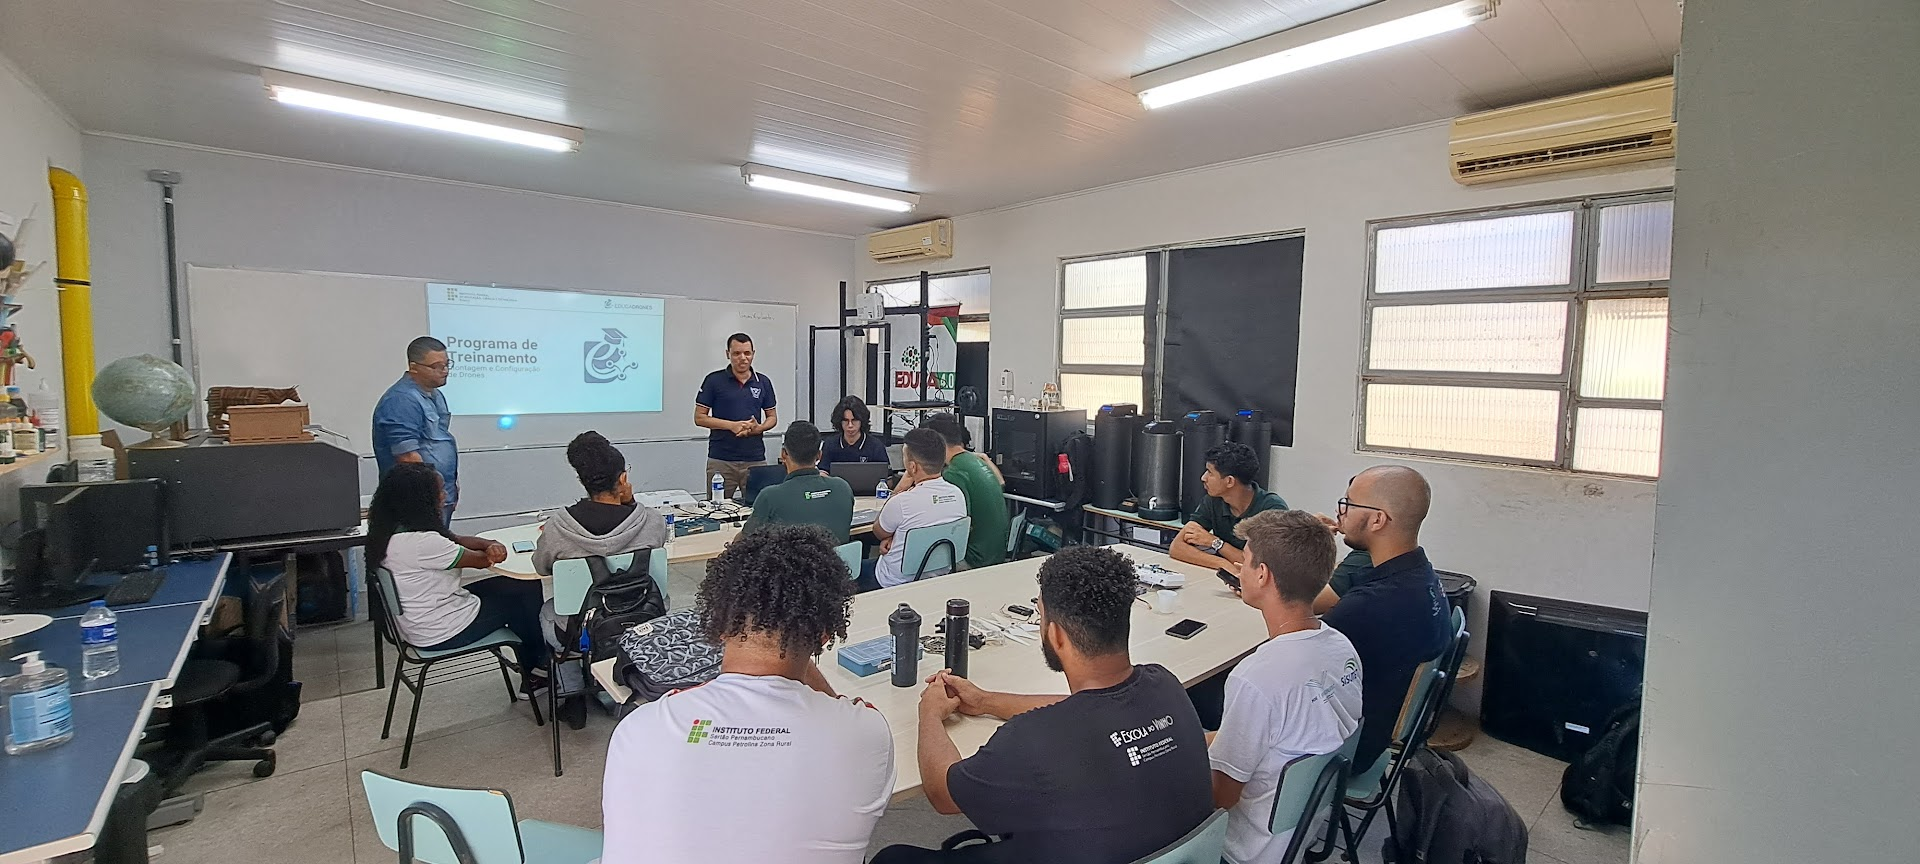
\includegraphics[scale=0.12]{img/petrolina.jpg} 
    \caption{Treinamento de Montagem e Configurações de Drones em Petrolina-PE. Fonte: Autor}
    \label{fig:petrolina}
\end{figure}

Entre essas iniciativas, destaca-se o programa de treinamento "Montagem e Configurações de Drones", oferecido pelo professor Leandro G. dos Santos, doutor em Agronomia, e por alunos do Educa Drones. O objetivo é fomentar a inovação em sistemas de aeronaves remotamente pilotadas (RPAS) nos diversos campi do IF Baiano, com implementações já realizadas nos campi de Catu-BA, Alagoinhas-BA, e Petrolina Zona Rural (figura \ref{fig:petrolina}), do Instituto Federal do Sertão Pernambucano. O curso também é regularmente oferecido no campus de origem, com planos de expandir para outros campi do IF Baiano e região.

Voltado para alunos do ensino médio e graduação, o curso adota a metodologia STEAM, abordando a legislação, aplicação, montagem e configuração de drones, integrando teoria e prática de forma didática.

Para manter o interesse dos participantes dos eventos promovidos pelo projeto, buscamos incentivar a participação em competições, como a Olimpíada Brasileira de Drones Aeromodelos, cuja primeira edição ocorrerá em 2025. Essas competições promovem a criação de inovações e o desenvolvimento científico no país.

\subsection{Aplicação em Competições}

\begin{figure}[!htb]
    \centering
    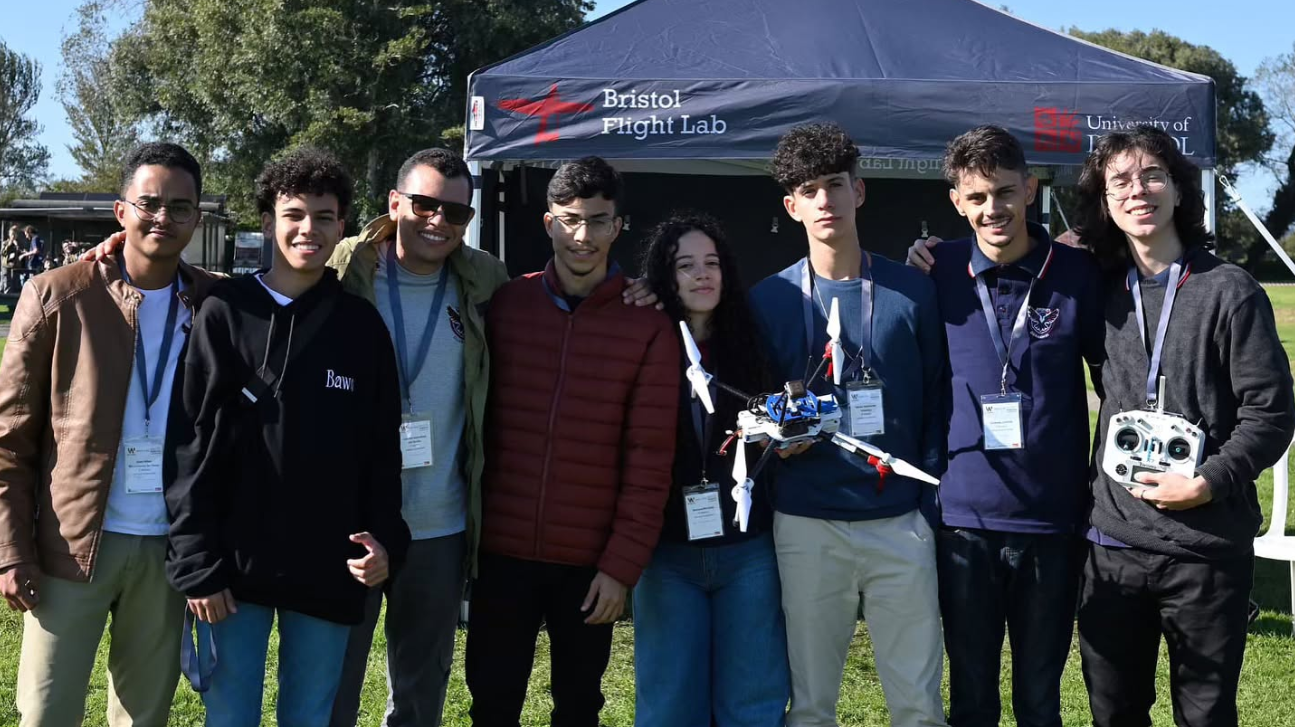
\includegraphics[scale=0.30]{img/imav2024.png} 
    \caption{Equipe Drones Guanambi na competição outdoor da IMAV. Fonte: Autor}
    \label{fig:petrolina}
\end{figure}

(Apenas tendo ideias por enquanto, reorganizar conteudo após)
Alguns dos modelos já foram testados em competições, como na \textit{International Micro Aerial Vehicles Competition} de 2024, onde o Colibri Standard (figura \ref{fig:ColibriStandard}) foi utilizado pela equipe Drones Guanambi

\section*{Considerações Finais}

O estudo destacou as características distintivas de cada modelo de drone desenvolvido no projeto Educa Drones, evidenciando suas aplicações ideais com base em peso, tempo de voo e capacidades de telemetria. O desenvolvimento contínuo e a avaliação desses drones podem levar a melhorias significativas na eficiência e versatilidade dos veículos aéreos não tripulados.

Para conclusões mais abrangentes, são necessários dados adicionais dos modelos Colibri Micro e Colibri Hexa. Investigações futuras devem focar na coleta desses dados, bem como nas análises de resistência, peso máximo de decolagem e estabilidade e voo em condições de vento adversas. Além disso, a comparação com outros drones comerciais pode fornecer uma perspectiva mais ampla sobre a competitividade dos modelos desenvolvidos.

\begin{thebibliography}{00}
\bibitem{b1} Abreu, J. V. V.; Bastos, B. L. (2015). Robótica Pedagógica e Currículo do Ensino Fundamental: Atuação em uma Escola Municipal do Projeto UCA. Revista Brasileira de Informática na Educação, v.23, n.3, 2015

\bibitem{b2} Brasil. Agência Nacional de Aviação Civil. (2023). Requisitos gerais para aeronaves não tripuladas de uso civil. RBAC-E94. Emenda n.3. Brasília, 2023.

\bibitem{b3} CBR, Competição Brasileira de Robótica. Disponível em: <https://cbr.robocup.org.br/index.php/categorias/> Acessado em de 30 junho 2024.

\bibitem{b4} IFSC, Competição de Drones IFSC Câmpus Florianópolis. Disponível em: <https://www.ifsc.edu.br/web/campus-florianopolis/veiculos-nao-tripulados-competicao-de-drones> Acessado em de 30 junho 2024.

\bibitem{b5} MNR, Mostra Nacional de Robótica. Disponível em: <https://mnr.robocup.org.br/> Acessado em de 30 junho 2024.

\bibitem{b6} OECD. PISA 2022 Results (Volume I): The State of Learning and Equity in Education. Paris: OCDE Publishing, 2023.

\bibitem{b7} SAE BRASIL. (2020). Fórmula Drone. Disponível em: <http://portal.saebrasil.org.br/programas-estudantis/sae-brasil-helidesign> Acesso: 20 de junho de 2020.

\bibitem{b8} Takagaki, L. K. (2012). Tecnologia de impressão 3D. Revista Inovação Tecnológica, São Paulo, v.2, n.2. p.2840. jul./dez.2012. 

\bibitem{b9} Ventura, A. A. O.; Albuquerque, J. L.; Praça Gomes, K. R. F.; Nascimento, S. M.; Leite, E. F.; Alves, J. L.; Diniz, J. R. B.; França, S. V. A. (2022). Robótica educacional e utilização de drones na educação: um mapeamento sistemático da literatura. Research, Society and Development, v. 11, n. 17, e251111739115, 2022.

\bibitem{b10} Wong, K. V.; Hernandez, A. A Review of Additive Manufacturing. ISRN Mechanical Engineering, v. 2012, p. 1–10, 2012

\bibitem{b11} Yepes, I. (2021). Uso de drones como Tecnologia pedagógica em disciplinas steam: um enfoque voltado ao aprendizado significativo com metodologias ativas. Tese (Doutorado) - Universidade Federal do Rio Grande do Sul, Centro de Estudos Interdisciplinares em Pós-Graduação em Informática na Educação. 2021, 240f. 

\bibitem{b12} Yepes, I.; Barone, D. A. C. (2018) Robótica Educativa: Proposta de uso de drones no apoio ao processo pedagógico em disciplinas STEM. Re, v(9). 2018. http://doi.org/10.5281/zenodo.1478926

\end{thebibliography}

\end{document}